\chapter{Natural Language ToolKit (NLTK)}

\nt{Dato che si parla di python avrei evitato di prendere appunti su questa merda, ma per completezza lo faccio lo stesso.}

\dfn{NLTK}{
  NLTK è un libro e una libreria di python che fornisce molti pacchetti di text processing e un gran numero di datasets. Permette di effettuare molto facilmente varie operazioni di tokenizzazione, parsing, stemming, etc.
}

\section{Introduzione ai Tasks di NLP}

\subsection{Tokenizzazione}

\dfn{Tokenizzazione}{
  Tokenizzare una stringa significa separarla in parole o frasi:
  \begin{itemize}
    \item Word tokenizzation: per identificare le parole, la più piccola unità di testo con un significato. 
    \item Sentence tokenizzation: un testo è diviso nelle frasi che contiene. 
  \end{itemize}
}

\begin{figure}[h]
    \centering
    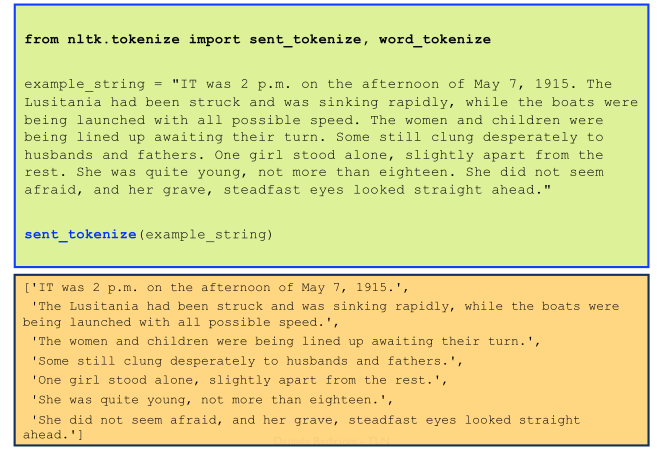
\includegraphics[scale=0.5]{04/n1.png}
    \caption{Tokenizzazione.}
\end{figure}

\subsection{Stop-Words Filtering}

\dfn{Stop-Words Filtering}{
  Alcune parole non hanno significato di per sé ma sono solo congiunzioni, in tal casi devono essere rimosse.
}

\clm{}{}{
  \begin{itemize}
    \item Le \fancyglitter{context words} forniscono informazioni sui topics presenti nell'articolo. 
    \item Caratterizzano lo stile di scrittura.
  \end{itemize}
}

\begin{figure}[h]
    \centering
    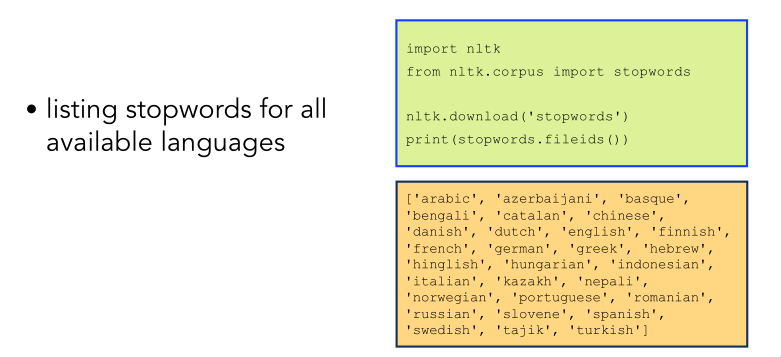
\includegraphics[scale=0.5]{04/n2.png}
    \caption{Meccanismo per elencare le Stop-Words.}
\end{figure}

\subsection{Stemming}

\dfn{Stemming}{
  Lo stemming consiste nel ridurre le parole alla loro radice ossia il nucleo delle parole.
}

\nt{Per esempio "Helping" e "Helper" condidono "Help".}

\paragraph{Possibili errori:}

\begin{itemize}
  \item \fancyglitter{Understemming:} due parole collegate dovrebbero essere ridotte alla stessa ma non lo sono. 
  \item \fancyglitter{Overstemming:} due parole non collegate sono ridotte alla stessa.
\end{itemize}

\begin{figure}[h]
    \centering
    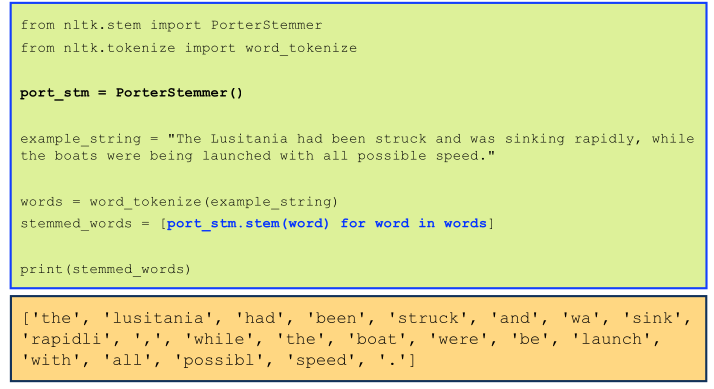
\includegraphics[scale=0.4]{04/n3.png}
    \caption{Stemming.}
\end{figure}

\begin{figure}[h]
    \centering
    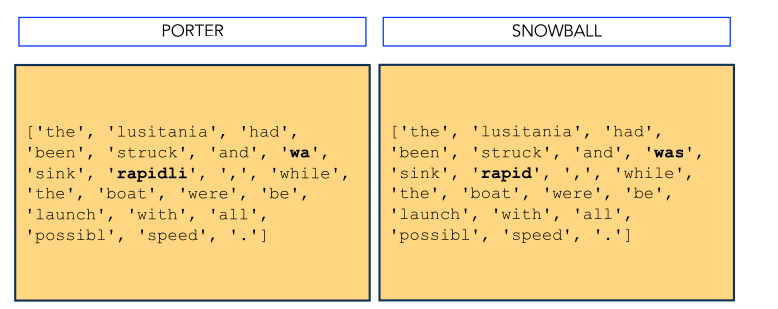
\includegraphics[scale=0.4]{04/n4.png}
    \caption{Confronto tra due stemmer di NLTK.}
\end{figure}

\subsection{PoS Tagging}

\dfn{Part of Speech Tagging}{
  Il Part of Speech Tagging è il task che consiste nell'etichettare le parole con la corrispettiva parte del discorso.
}

\begin{figure}[h]
    \centering
    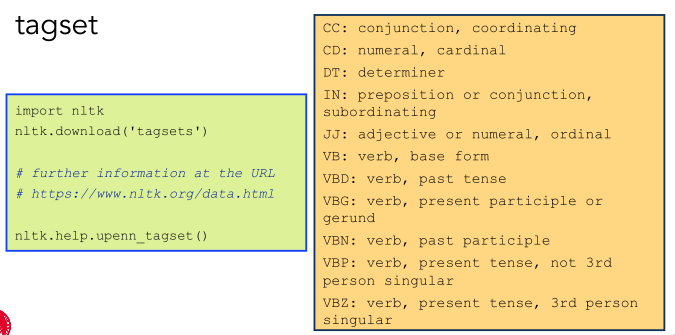
\includegraphics[scale=0.4]{04/n5.png}
    \caption{Tagset.}
\end{figure}

\subsection{Lemmatizzazione}

\dfn{Lemmatizzazione}{
La lemmatizzazione riduce le parole alla loro forma canonica (lemma).
}

\cor{Lemma}{
  Un lemma è la forma canonica che si può trovare nel dizionario. Un lemma è una parola che rappresenta un intero gruppo di parole chiamato lessema.
}

\begin{figure}[h]
    \centering
    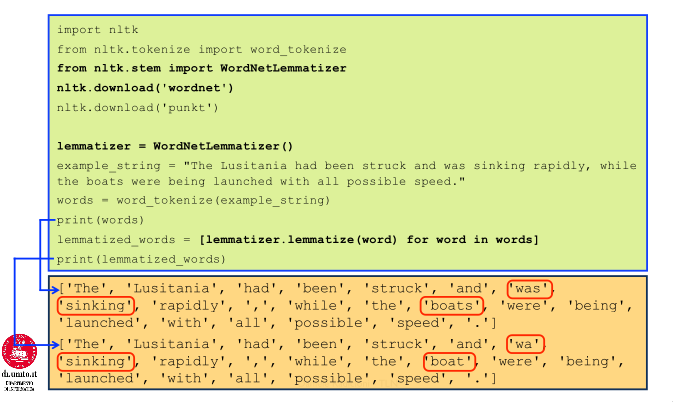
\includegraphics[scale=0.4]{04/n6.png}
    \caption{Lemmatizzazione.}
\end{figure}

\nt{La performance di un lemmatizer può essere aumentata aggiungendo PoS tagging.}

\subsection{NER}

\dfn{Named Entity Recognition}{
  Named Entities sono frasi con nomi che si riferiscono a specifiche località, persone, organizzazioni, etc. Il task NER consiste nel trovare le Named Entities in un testo e determinarne il tipo.
}

\section{SpaCy}

\dfn{SpaCy}{
  SpaCy è una libreria opensource per NLP in python. Offre varie funzioni:
  \begin{itemize}
    \item Tokenizzazione. 
    \item PoS tagging. 
    \item Lemmatizzazione. 
    \item Parsing a dipendenze. 
    \item Sentence Boundary Detection (SBD). 
    \item NER.
  \end{itemize}
}

\paragraph{Funzionalità avanzate:}

\begin{itemize}
  \item Entity linking: disambiguare entità testuali in identificatori univoci in unabase di conoscenza. 
  \item Similarity: comparare parole, testi, documenti, etc. 
  \item Text classification: assegnare categorie o etichette a un documento o a parti di esso.
  \item Matching a regole: trovare sequenze di token basandosi su annotazioni linguistiche (simile alle regex). 
  \item Training: aggiornare e migliorare predizioni di modelli statistici. 
  \item Serializzazione: salvare oggetti in file o byte.
\end{itemize}

\cor{Modello}{
  Alcune features di SpaCy sono indipendenti, mentre altre richiedono una pipeline per essere caricate. Una pipeline addestrata  consiste di molteplici componenti che usano modelli statistici su dati etichettati.
}

\nt{Sono inclusi diversi linguaggi.}

\cor{Annotazioni Linguistiche}{
  Le annotazioni linguistiche offrono una visione delle strutture grammaticali e sintattiche. 
}

\subsection{La Pipeline}

Chiamando \texttt{nlp} su un testo SpaCy effettua tokenizzazione, altri processi e infine restituisci in output un \texttt{Doc}.

\begin{figure}[h]
    \centering
    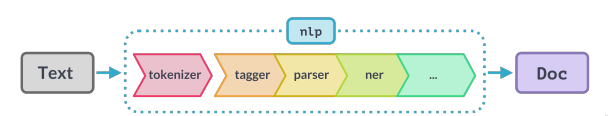
\includegraphics[scale=0.4]{04/n7.png}
    \caption{La pipeline.}
\end{figure}

\begin{figure}[h]
    \centering
    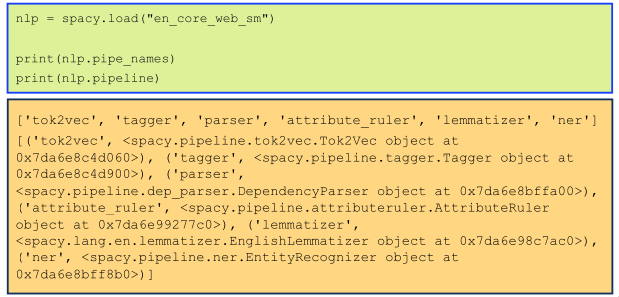
\includegraphics[scale=0.6]{04/n8.png}
    \caption{Ottenere informazioni sulla pipeline di SpaCy.}
\end{figure}

\nt{Nel processare grandi volumi di testo questi modelli sono più efficienti con insiemi di testi.}

\clm{}{}{
  \begin{itemize}
    \item Per aumentare la velocità si può scegliere di disabilitare o escludere una parte della pipeline. 
    \item \texttt{disable:} i componenti sono caricati, ma non utilizzati. 
    \item \texttt{exclude:} i componenti non sono caricati.
  \end{itemize}
}

